\subsection{
    Комплексная плоскость, модуль, аргумент.
}

\begin{definition}
    \textbf{\textit{Комплексной плоскостью}} называется плоскость, образованная комплексными числами, у которой ось $Ox$ образована действительными числами, а ось $Oy$ - мнимыми числами.
\end{definition}

\begin{figure}[H]
    \centering
    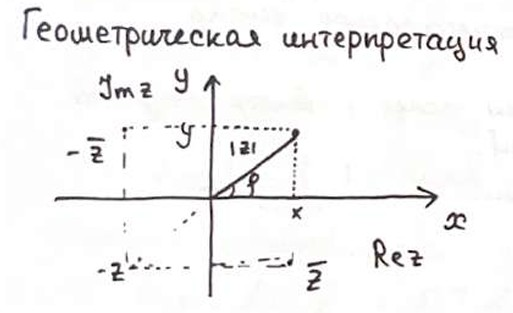
\includegraphics[scale=0.55]{images/module1/question01/1.jpg}
    \label{fig:picture_01_1}
\end{figure}


\begin{definition}
    \textbf{\textit{Модулем числа $z = x + iy$}} называется вещественное число $|z| = \sqrt{x^2 + y^2}$ (то есть длина соответствующего вектора).
\end{definition}

\textbf{Свойства.}

\begin{enumerate}[label={\arabic*°.}]
    \item $|z| \geq 0$, причем $|z| = 0 \iff z = 0$.
    \item $|z + w| \leq |z| + |w|$ (неравенство треугольника).

    Пусть $z = a + bi$, $w = c + di$.
    \begin{align*}
        |z + w| &\leq |z| + |w| \\
        \sqrt{(a + c)^2 + (b + d)^2} &\leq \sqrt{a^2 + b^2} + \sqrt{c^2 + d^2} \\
        (a + c)^2 + (b + d)^2 &\leq a^2 + b^2 + c^2 + d^2 + 2\sqrt{(a^2 + b^2)(c^2 + d^2)} \\
        ac + bd &\leq\sqrt{(a^2 + b^2)(c^2 + d^2)} \\
        ac + bd &\leq\sqrt{(ac)^2 + (ad)^2 + (bc)^2 + (bd)^2} \\
        (ac)^2 + (bd)^2 + 2acbd &\leq (ac)^2 + (ad)^2 + (bc)^2 + (bd)^2 \\
        2acbd &\leq (ad)^2 + (bc)^2 \\
        0 &\leq (ad)^2 + (bc)^2 - 2abcd \\
        0 &\leq (ad - bc)^2
    \end{align*}
    \item $z \overline{z} = |z|^2$.

    $z \overline{z} = (a + bi)(a - bi) = a^2 - (bi)^2 = a^2 + b^2 = |z|^2$
    \item $|zw| = |z||w|$.

    $|zw|^2 = (zw) \cdot (\overline{zw}) = z \cdot w \cdot \overline{z} \cdot \overline{w} = |z|^2 |w|^2$.
\end{enumerate}


\subsubsection*{
    Аргумент комплексного числа.
}


Пусть $z = a + bi \in \CC$, $z \neq 0$.

Тогда, $z = |z| \left(\frac{a}{|z|} + \frac{b}{|z|}i\right)$, при этом $\left(\frac{a}{|z|}\right)^2 + \left(\frac{b}{|z|}\right)^2 = (\frac{a}{\sqrt{a^2 + b^2}})^2 + (\frac{b}{\sqrt{a^2 + b^2}})^2 = \frac{a^2}{a^2 + b^2} + \frac{b^2}{a^2 + b^2} = \frac{a^2 + b^2}{a^2 + b^2} = 1.$

Значит, $\frac{a}{|z|}$ и $\frac{b}{|z|}$ являются синусом и косинусом некоторого угла.

\begin{definition}
    \textbf{\textit{Аргументом числа}} $z = a + bi \in \CC \setminus \{0\}$ называется любое число $\phi \in \RR$, такое что
    \begin{equation*}
        \cos \phi = \frac{a}{|z|} = \frac{a} {\sqrt{a^2 + b^2}}.
    \end{equation*}

    \begin{equation*}
        \sin \phi = \frac{b}{|z|} = \frac{b}{\sqrt{a^2 + b^2}}.
    \end{equation*}

    В геометрических терминах, $\phi$ есть угол между положительным направлением оси $Ox$ и вектором с началом в точке $0$ и концом в точке $z$.
\end{definition}

\begin{comment}
    Таких чисел бесконесно много, причем такие числа отличаются на $2\pi k, k \in \ZZ$.
\end{comment}
